\documentclass[UTF8,a4paper,12pt]{ctexart}

\usepackage{geometry}
\usepackage{amsmath,amssymb,bm}
\usepackage{booktabs,longtable,array,multirow}
\usepackage{graphicx}
\usepackage{caption}
\usepackage{subcaption}
\usepackage{enumitem}
\usepackage{float}
\usepackage{hyperref}
\usepackage{xcolor}

\geometry{left=2.55cm,right=2.55cm,top=2.55cm,bottom=2.55cm}
\setlength{\parindent}{2em}
\setlength{\parskip}{0.12em}
\linespread{1.12}
\graphicspath{{figures/}}

\hypersetup{colorlinks=true,linkcolor=black,citecolor=black,urlcolor=black}

\ctexset{
  section = {format = \zihao{4}\bfseries},
  subsection = {format = \zihao{-4}\bfseries},
  subsubsection = {format = \zihao{-4}\bfseries}
}

\captionsetup{font=small,labelfont=bf}
\renewcommand{\arraystretch}{1.12}
\setlist{nosep,leftmargin=2em}

\newcommand{\NHthree}{\mathrm{NH_3}}
\newcommand{\Htwo}{\mathrm{H_2}}
\newcommand{\MWh}{\mathrm{MWh}}
\newcommand{\MW}{\mathrm{MW}}
\newcommand{\Rself}{R^{self}}
\newcommand{\Rgreen}{R^{green}}
\newcommand{\Rsell}{R^{sell}}

\begin{document}

% ===================== 第 1 页：封面页 =====================
\begin{titlepage}
  \thispagestyle{empty}
  \centering
  \vspace*{2.0cm}
  {\zihao{2}\bfseries 2026年电工杯数学建模竞赛论文\par}
  \vspace{2.0cm}
  {\zihao{1}\bfseries A题\par}
  \vspace{0.8cm}
  {\zihao{2}\bfseries 绿电直连型电氢氨园区优化运行\par}
  \vfill
  \begin{tabular}{>{\bfseries}rl}
    参赛编号： & \underline{\hspace{6cm}} \\
    论文题目： & 绿电直连型电氢氨园区优化运行 \\
    提交文件： & PDF论文与支撑材料压缩包 \\
  \end{tabular}
  \vfill
  {\zihao{4}本文不设置目录；题目、摘要、关键词位于第2页，正文自第3页开始。\par}
\end{titlepage}

% ===================== 第 2 页：题目、摘要、关键词 =====================
\clearpage
\setcounter{page}{2}
\thispagestyle{plain}

\begin{center}
  {\zihao{2}\bfseries 绿电直连型电氢氨园区优化运行\par}
\end{center}

\vspace{0.4em}
\noindent\textbf{摘要：}
绿电直连模式通过新能源电源与高载能产业负荷直接耦合，可促进新能源就近消纳并推动化工行业低碳转型，但风光出力波动与制氢制氨负荷之间的时序错配会引发购电、上网、弃电和系统备用成本等问题。针对绿电直连型电氢氨园区优化运行问题，本文建立了从刚性基准、离散开停、连续调节到离网储能配置的小时级优化模型，并进一步基于计算结果分析绿电直连高渗透对电力系统的影响。

首先，针对典型日刚性满负荷运行，建立并网功率平衡、三项绿电指标和题面成本口径下的吨氨成本模型。结果表明，典型日新能源自发自用比例为64.08\%，总用电量绿电比例为69.21\%，均满足要求；但新能源上网比例为35.92\%，超过20\%约束，说明固定负荷难以主动匹配风光出力。其次，扩容至72 t/d后，构建离散开停机模型，并用边际成本排序法求解。典型场景下，若要求三项绿电指标全部满足，54 t/d为最低成本可行方案，吨氨成本为4591.27元/t；24场景年度统计显示，降低日产量虽可降本，但会提高上网比例并削弱绿电指标合规性。进一步地，建立连续制氨负荷率混合整数线性规划模型，引入购售电互斥约束以避免非物理套利。连续调节使36 t/d方案较离散开停降本284.35元/t，并将全年全满足代表天数由0天提高至165天，表明柔性负荷可显著改善源荷时序匹配。

在离网运行场景下，本文删除购售电变量，引入储能充放电、SOC动态、弃风弃光和常规负荷缺供变量，建立离网储能调度模型。结果显示，无储能离网年产氨量为9781.56 t，产能利用率仅37.74\%，年弃电14188.67 MWh；配置5 MWh储能后常规负荷缺供降为0，年弃电降至11280.74 MWh。进一步的储能经济--消纳Pareto分析表明，5 MWh为经济方案，若最大弃电场景弃电率不超过10\%需80 MWh，零弃电需155 MWh。并网同产量对比表明，公共电网支撑价值为735.81元/t。最后，本文据此提出小时级绿电溯源、上网比例与最大交换功率考核、柔性负荷准入补偿、储能多目标评估和系统费用分担等建议。

\vspace{0.6em}
\noindent\textbf{关键词：}
绿电直连；电氢氨园区；合成氨负荷调节；储能配置；混合整数线性规划；新能源消纳

% ===================== 正文：第 3 页开始，不设目录 =====================
\clearpage
\setcounter{page}{3}

\section{问题背景与重述}

\subsection{问题背景}

在高比例新能源接入背景下，风电、光伏出力的波动性与工业负荷的连续性之间存在显著矛盾。绿电直连通过将新能源电源与电解制氢、合成氨等高载能负荷在园区层面耦合，为新能源就地消纳和化工行业低碳转型提供了新的实现路径。然而，若园区只按年累计电量平衡进行设计，可能掩盖小时尺度上的源荷错配，导致部分时段向公共电网购电，另一些时段又向外部电网反送电。对于电氢氨园区，制氢电解槽、合成氨装置、储能和公共电网共同构成多能耦合系统，其运行优化需要同时兼顾功率平衡、制氨产量、绿电指标、吨氨成本和电力系统友好性。

\subsection{问题重述}

题目给定园区常规负荷曲线、典型日风光出力、24种风光组合场景、风光发电成本、分时电价、余电上网价格、电解槽与合成氨设备参数以及储能参数。需要完成如下任务：第一，计算典型日固定制氢制氨负荷下的购电量、上网电量、绿电指标和吨氨成本；第二，扩容至72 t/d后，考虑制氨装置离散开停机并优化不同日产量下的运行时段；第三，将制氨负荷放宽为10\%--100\%连续可调，并与离散开停机模型对比；第四，在离网条件下引入储能，分析弃风弃光、缺供风险、储能容量和并网同产量经济性；第五，基于前四问结果，分析绿电直连园区高渗透对新能源消纳、电网调峰、备用、费用分担和政策机制的影响。

\section{问题分析}

五个问题构成逐步增加系统柔性的递进链条。问题一不进行优化，作为刚性满负荷运行基准，用于识别源荷错配和指标不达标环节。问题二在扩容后引入离散开停机变量，通过选择生产时段改善经济性和消纳指标。问题三进一步将开停机模式放宽为连续负荷率调节，并引入购售电互斥约束，量化柔性负荷价值。问题四切换到离网运行，删除购售电变量，引入储能和缺供变量，用于评价完全依赖风光时的可靠性与成本。问题五不再新增调度优化变量，而是将前四问结果组织为证据矩阵，讨论绿电直连对外部电力系统和政策机制的影响。

从数学结构看，问题一是确定性核算模型；问题二由于缺少启停成本和爬坡约束，可转化为边际成本排序问题；问题三和问题四涉及连续变量与二进制互斥变量，采用混合整数线性规划求解；问题五则是基于模型输出的证据化政策分析。本文由此形成“指标核算--运行优化--储能配置--系统影响”的完整分析框架。

\section{模型假设}

\begin{enumerate}[label=\textbf{H\arabic*}.]
  \item 以小时为基本调度时间尺度，令$\Delta t=1$ h。
  \item 问题二至四的24种风光组合场景由6种风电场景和4种光伏场景组合得到，每个场景代表15天，全年按360天加权统计。
  \item 并网问题中新能源自发自用电量采用主口径$E^{self}=E^{re}-E^{sell}$，题面括号公式仅作为复核口径。
  \item 扩容后72 t/d工况下，碱性电解槽、PEM电解槽和合成氨装置聚合为同步产氢--制氨单元，满负荷功率为41.5 MW，满负荷产氨能力为3 t/h。
  \item 成本均为题面成本口径下的比较成本，包含风光发电成本、购电成本、余电上网收益、设备运维和储能年化成本，不包含未给定参数的全寿命固定投资。
  \item 储能按1C配置，即$P^{cap}=E^{cap}$；储能SOC采用典型日闭环约束。
  \item 不考虑电网潮流、电压、无功、短路容量等配网约束；不考虑合成氨反应器热惯性、启停成本、最小开停时间和氢氨储罐动态。
\end{enumerate}

\section{符号说明与数据处理}

\subsection{符号说明}

\begin{longtable}{p{0.24\textwidth}p{0.64\textwidth}}
\toprule
符号 & 含义 \\
\midrule
\endhead
$s,t,D$ & 风光组合场景、小时编号、日产氨量目标 \\
$P^w_{s,t},P^{pv}_{s,t},P^{re}_{s,t}$ & 风电、光伏和新能源总出力，单位MW \\
$P^L_t$ & 园区常规电负荷，单位MW \\
$u_{s,D,t},y_{s,D,t}$ & 连续制氨负荷率、离散开停机变量 \\
$P^{buy}_{s,t},P^{sell}_{s,t}$ & 购电功率和上网功率，单位MW \\
$P^{cur}_{s,t},P^{shed}_{s,t}$ & 弃风弃光功率、常规负荷缺供功率，单位MW \\
$P^{ch}_{s,t},P^{dis}_{s,t},E_{s,t}$ & 储能充电功率、放电功率和SOC \\
$M^{\NHthree},C,LCOA$ & 产氨量、总成本和题面成本口径下的吨氨成本 \\
$\Rself,\Rgreen,\Rsell$ & 新能源自发自用比例、总用电量绿电比例和新能源上网比例 \\
$R^{cur},R^{use}$ & 弃风弃光率和风光利用率 \\
\bottomrule
\end{longtable}

\subsection{数据说明及预处理}

本文使用题目附件1--8。问题一采用附件1和附件2构成典型日；问题二至四将6种风电场景与4种光伏场景组合，形成24种风光场景。每个组合场景代表15天，年度统计采用
\[
X^{year}=\sum_{s=1}^{24}15X_s .
\]
常规负荷由附件1标幺曲线乘以6 MW得到。问题一采用初始制氨能力36 t/d，生产单元满负荷功率为
\[
P^{prod}=10+10+0.75=20.75\ {\rm MW},\quad q^{\NHthree}=1.5\ {\rm t/h}.
\]
问题二至四采用扩容后72 t/d能力：
\[
P^{prod}=20+20+1.5=41.5\ {\rm MW},\quad q^{\NHthree}=3\ {\rm t/h}.
\]
此时合成氨每小时需氢600 kg，两类电解槽满负荷产氢量为$280+320=600$ kg/h，故可将制氢和合成氨聚合为同步生产单元。

\section{统一模型框架}

\subsection{并网功率平衡与绿电指标}

并网运行下，园区小时功率平衡为
\[
P^{re}_{s,t}+P^{buy}_{s,t}=P^L_t+P^{prod}_{s,t}+P^{sell}_{s,t}.
\]
并网型绿电直连指标按
\[
E^{self}=E^{re}-E^{sell},\qquad
\Rself=\frac{E^{self}}{E^{re}},\quad
\Rgreen=\frac{E^{self}}{E^{load}},\quad
\Rsell=\frac{E^{sell}}{E^{re}}
\]
计算，并与$60\%$、$30\%$和$20\%$阈值比较。题面括号公式$E^{load}-E^{sell}-E^{buy}$作为复核口径保留。

\subsection{成本核算模型}

日净成本统一写为
\[
C=C^w+C^{pv}+C^{buy}+C^{om}+C^{bat}-I^{sell}.
\]
其中$C^w$、$C^{pv}$为风电和光伏发电成本，$C^{buy}$为分时购电成本，$C^{om}$为电解槽和合成氨装置运维成本，$C^{bat}$为储能成本，$I^{sell}$为余电上网收益。吨氨成本为
\[
LCOA=\frac{C}{M^{\NHthree}}.
\]
本文的$LCOA$均为题面成本口径下的比较成本，不代表包含全部固定投资的工程全寿命平准化成本。

\section{问题一：典型日刚性满负荷运行指标核算}

\subsection{模型建立}

在问题一中，制氢制氨负荷全天满负荷运行，工艺负荷为20.75 MW，日产氨量为36 t。对每个小时直接由功率平衡得到
\[
P^{buy}_t=\max(P^L_t+20.75-P^{re}_t,0),
\]
\[
P^{sell}_t=\max(P^{re}_t-P^L_t-20.75,0).
\]
随后按统一绿电指标和成本模型计算典型日结果。

\subsection{结果分析}

\begin{table}[H]
\centering
\caption{问题一典型日核心结果}
\label{tab:q1_result}
\small
\begin{tabular}{l r@{\quad}l}
\toprule
指标 & 数值 & 单位 \\
\midrule
典型日总用电量 & 558.7200 & MWh \\
新能源发电量 & 603.4480 & MWh \\
网购电量 & 172.0438 & MWh \\
上网电量 & 216.7718 & MWh \\
新能源自发自用比例 & 64.08 & \% \\
总用电量绿电比例 & 69.21 & \% \\
新能源上网电量比例 & 35.92 & \% \\
吨氨成本 & 4322.34 & 元/t \\
\bottomrule
\end{tabular}
\end{table}

\begin{figure}[H]
  \centering
  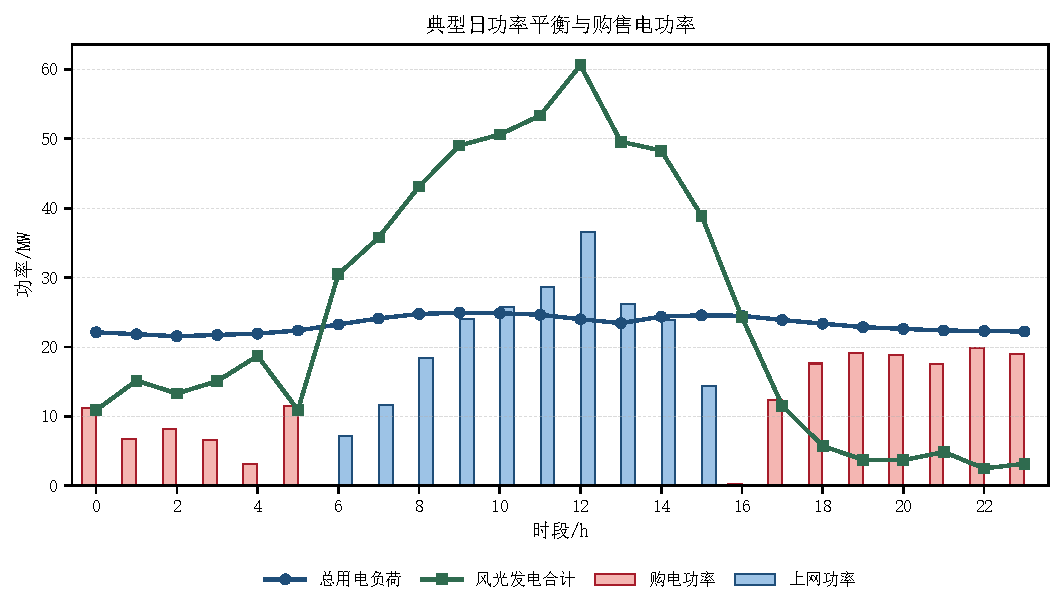
\includegraphics[width=0.88\textwidth]{fig01_q1_power_balance.pdf}
  \caption{典型日风光出力、园区负荷与电网交换功率}
  \label{fig:q1_power_balance}
\end{figure}

由表\ref{tab:q1_result}可知，典型日自发自用比例和绿电比例均满足要求，但新能源上网比例为35.92\%，超过20\%约束。图\ref{fig:q1_power_balance}表明，夜间光伏出力为零且风电不足时需要购电，白天风光出力集中时又产生大量上网电量。该结果说明，刚性制氨负荷无法主动追踪风光出力变化，是后续负荷调节和储能配置的直接动因。

\begin{figure}[H]
  \centering
  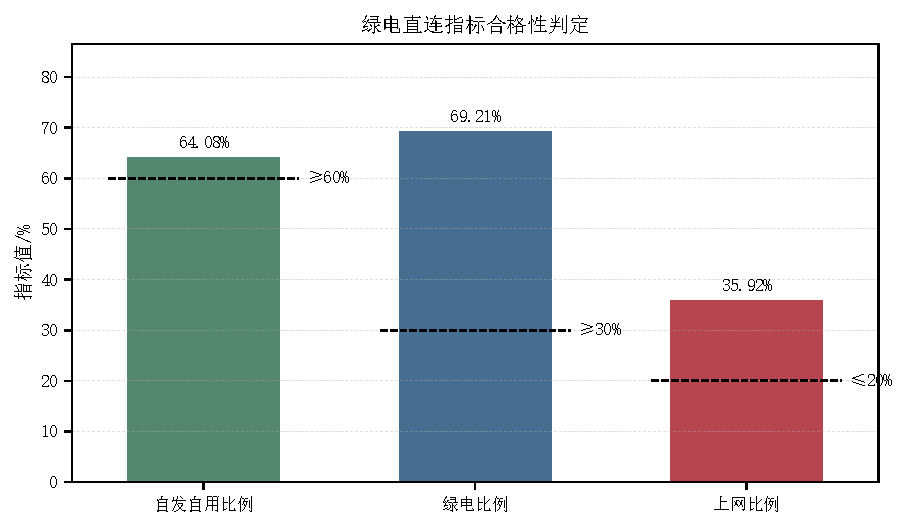
\includegraphics[width=0.74\textwidth]{fig02_q1_indicator_check.pdf}
  \caption{问题一三项绿电指标达标情况}
  \label{fig:q1_indicator}
\end{figure}

\section{问题二：离散开停机制氨调节优化}

\subsection{模型建立}

扩容后聚合生产单元满负荷功率为41.5 MW，满负荷产氨能力为3 t/h。设$y_{s,D,t}\in\{0,1\}$表示场景$s$、日产量$D$、时段$t$是否满负荷开机，则
\[
P^{prod}_{s,D,t}=41.5y_{s,D,t},\qquad
m^{\NHthree}_{s,D,t}=3y_{s,D,t}.
\]
日产量集合取
\[
D\in\{72,63,54,45,36\}\ {\rm t/d},
\]
对应开机小时数
\[
H_D=\frac{D}{3}\in\{24,21,18,15,12\}.
\]
约束为
\[
\sum_{t=1}^{24}y_{s,D,t}=H_D.
\]
对给定场景和日产量，目标为最小化日净成本：
\[
\min C_{s,D}=C^w_s+C^{pv}_s+C^{buy}_{s,D}+C^{om}_{s,D}-I^{sell}_{s,D}.
\]

\subsection{边际成本排序法}

由于题面未给定启停成本、最小开机时间和爬坡约束，各时段之间仅通过总开机小时数耦合。定义时段$t$由停机变为开机的边际成本：
\[
\Delta C_{s,t}=G_{s,t}(P^L_t+41.5)-G_{s,t}(P^L_t)+C^{om,h},
\]
其中
\[
G_{s,t}(P)=1000\left[c^{buy}_t\max(P-P^{re}_{s,t},0)-c^{sell}\max(P^{re}_{s,t}-P,0)\right].
\]
将24个小时的$\Delta C_{s,t}$从小到大排序，选择前$H_D$个时段开机即可得到全局最优解。

\subsection{求解结果}

典型风光场景结果见表\ref{tab:q2_typical}。若只看成本，36 t/d方案最低；若要求三项绿电指标全部满足，54 t/d方案是最低成本可行方案，吨氨成本为4591.27元/t。

\begin{table}[H]
\centering
\caption{问题二典型场景离散开停机结果}
\label{tab:q2_typical}
\small
\begin{tabular}{c c c c c c}
\toprule
日产量 & 开机小时 & 吨氨成本 & 自发自用 & 绿电比例 & 合格性 \\
/(t/d) & /h & /(元/t) & 比例 &  &  \\
\midrule
72 & 24 & 6219.14 & 93.26\% & 53.26\% & 全满足 \\
63 & 21 & 5328.06 & 92.17\% & 59.66\% & 全满足 \\
54 & 18 & 4591.27 & 90.08\% & 67.30\% & 全满足 \\
45 & 15 & 3944.54 & 75.49\% & 66.67\% & 部分满足 \\
36 & 12 & 3191.67 & 55.25\% & 59.68\% & 部分满足 \\
\bottomrule
\end{tabular}
\end{table}

24场景年度加权结果见表\ref{tab:q2_annual}。日产量越低，吨氨成本越低，但年上网电量显著增加，导致全满足天数下降。

\begin{table}[H]
\centering
\caption{问题二24场景年度加权结果}
\label{tab:q2_annual}
\small
\begin{tabular}{c r r r r r}
\toprule
日产量 & 年产氨 & 年均吨氨成本 & 年购电量 & 年上网量 & 全满足天数\\
/(t/d) & /t & /(元/t) & /MWh & /MWh & /d\\
\midrule
72 & 25920 & 7182.67 & 221146.80 & 12078.72 & 270 \\
63 & 22680 & 6523.27 & 183462.13 & 19214.05 & 210 \\
54 & 19440 & 5909.66 & 150249.86 & 30821.78 & 210 \\
45 & 16200 & 5290.32 & 127977.50 & 53369.41 & 15 \\
36 & 12960 & 4493.82 & 107277.55 & 77489.47 & 0 \\
\bottomrule
\end{tabular}
\end{table}

问题二说明，单纯降低日产量可以降低购电压力和吨氨成本，但也会降低本地负荷对新能源的吸纳能力，使余电上网比例升高。因此，成本最优与指标合规之间存在明显权衡。

\section{问题三：连续可调制氨负荷优化}

\subsection{模型建立}

设$u_{s,D,t}$为连续负荷率。主模型采用连续运行假设：
\[
0.1\le u_{s,D,t}\le 1,
\]
并满足日产量约束
\[
\sum_{t=1}^{24}3u_{s,D,t}=D.
\]
生产负荷为
\[
P^{prod}_{s,D,t}=41.5u_{s,D,t}.
\]
并网功率平衡为
\[
P^{re}_{s,t}+P^{buy}_{s,D,t}=P^L_t+41.5u_{s,D,t}+P^{sell}_{s,D,t}.
\]
为避免同一时段购电并售电的非物理套利，引入二进制变量$b_{s,D,t}$：
\[
P^{buy}_{s,D,t}\le Mb_{s,D,t},\qquad
P^{sell}_{s,D,t}\le M(1-b_{s,D,t}).
\]
目标函数为
\[
\min C_{s,D}=C^w_s+C^{pv}_s+C^{buy}_{s,D}+C^{om}_{s,D}-I^{sell}_{s,D}.
\]
该模型为小规模混合整数线性规划，本文采用SciPy HiGHS求解。

\subsection{结果与对比}

典型场景下，连续调节与离散开停具有相同日产量集合。54 t/d仍是满足三项指标的最低成本典型方案，吨氨成本为4530.88元/t。年度结果见表\ref{tab:q3_annual}。

\begin{table}[H]
\centering
\caption{问题三24场景年度加权结果}
\label{tab:q3_annual}
\small
\begin{tabular}{c r r r r r r}
\toprule
日产量 & 年产氨 & 年均吨氨成本 & 年购电量 & 年上网量 & 上网比例 & 全满足天数\\
/(t/d) & /t & /(元/t) & /MWh & /MWh & & /d\\
\midrule
72 & 25920 & 7182.67 & 221146.80 & 12078.72 & 7.05\% & 270 \\
63 & 22680 & 6413.13 & 176326.80 & 12078.72 & 7.05\% & 300 \\
54 & 19440 & 5663.95 & 137231.50 & 17803.42 & 10.39\% & 240 \\
45 & 16200 & 5008.76 & 109563.64 & 34955.56 & 20.40\% & 240 \\
36 & 12960 & 4209.48 & 91060.62 & 61272.54 & 35.76\% & 165 \\
\bottomrule
\end{tabular}
\end{table}

与问题二相比，连续调节在除72 t/d外的所有日产量下均降低年均吨氨成本，见表\ref{tab:q2q3_compare}。36 t/d方案降本284.35元/t，45 t/d方案全满足天数由15天提高到240天，说明连续可调负荷能够显著改善源荷时序匹配。

\begin{table}[H]
\centering
\caption{问题二与问题三年度结果对比}
\label{tab:q2q3_compare}
\small
\begin{tabular}{c r r r r}
\toprule
日产量/(t/d) & Q2成本 & Q3成本 & 降本/(元/t) & 全满足天数变化\\
\midrule
72 & 7182.67 & 7182.67 & 0.00 & 0 \\
63 & 6523.27 & 6413.13 & 110.15 & +90 \\
54 & 5909.66 & 5663.95 & 245.71 & +30 \\
45 & 5290.32 & 5008.76 & 281.55 & +225 \\
36 & 4493.82 & 4209.48 & 284.35 & +165 \\
\bottomrule
\end{tabular}
\end{table}

\begin{figure}[H]
  \centering
  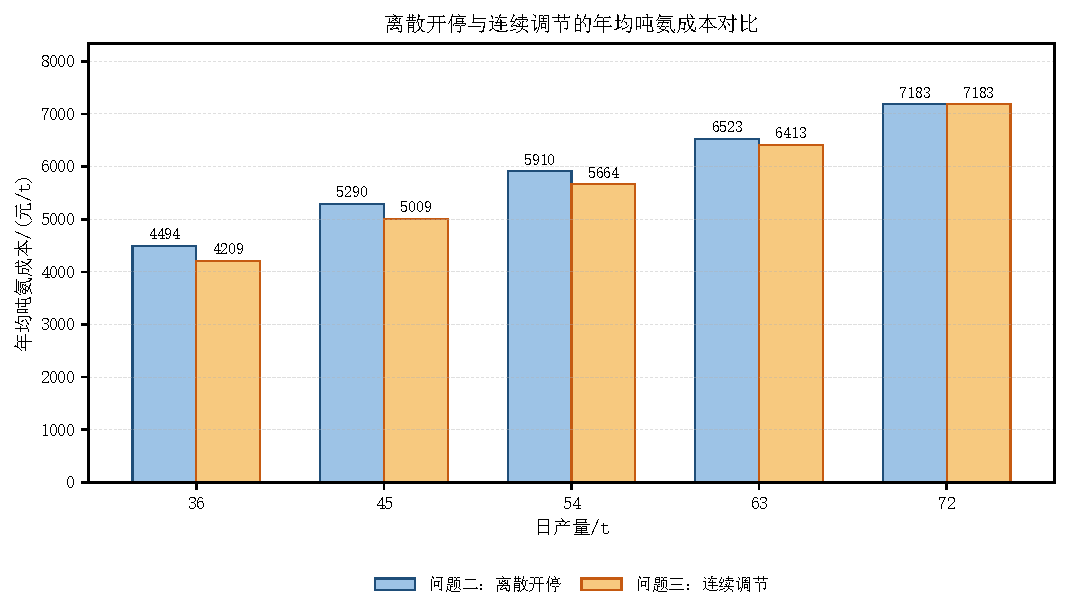
\includegraphics[width=0.78\textwidth]{fig03_q2_q3_cost_compare.pdf}
  \caption{离散开停机与连续调节的年均吨氨成本对比}
  \label{fig:q2q3_cost}
\end{figure}

\begin{figure}[H]
  \centering
  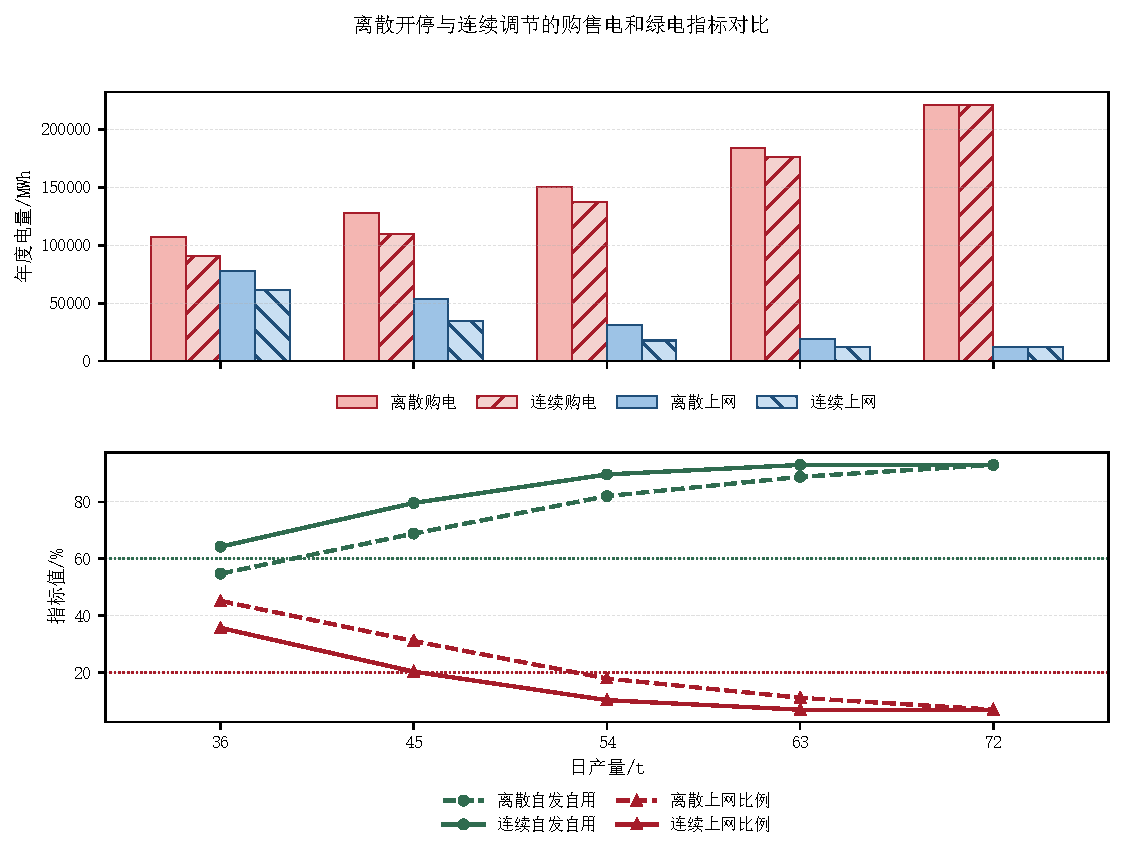
\includegraphics[width=0.86\textwidth]{fig04_q2_q3_grid_indicator.pdf}
  \caption{离散开停机与连续调节的电网交换和指标对比}
  \label{fig:q2q3_grid}
\end{figure}

72 t/d因全天满负荷运行，连续模型没有调节自由度，结果与离散模型一致。中低日产量下，连续负荷率可在风光富余或电价较低时提高负荷，在风光不足或电价较高时降低负荷，从而同步减少购电和上网。

\section{问题四：离网运行与储能配置优化}

\subsection{无储能离网模型}

离网运行取消外部购售电。无储能时功率平衡为
\[
P^w_{s,t}+P^{pv}_{s,t}+P^{shed}_{s,t}
=P^L_t+41.5u_{s,t}+P^{cur}_{s,t}.
\]
若风光扣除常规负荷后的可用功率低于制氨10\%运行下限，则制氨停机；若风光不足以满足常规负荷，则记录缺供。离网部分不再计算上网比例，而采用
\[
R^{use}_s=\frac{E^{re}_s-E^{cur}_s}{E^{re}_s},\qquad
R^{cur}_s=\frac{E^{cur}_s}{E^{re}_s}.
\]

\subsection{含储能离网模型}

引入储能后，离网功率平衡为
\[
P^w_{s,t}+P^{pv}_{s,t}+P^{dis}_{s,t}+P^{shed}_{s,t}
=P^L_t+41.5u_{s,t}+P^{ch}_{s,t}+P^{cur}_{s,t}.
\]
储能SOC动态为
\[
E_{s,t}=(1-\rho)E_{s,t-1}+\eta^{ch}P^{ch}_{s,t}
-\frac{P^{dis}_{s,t}}{\eta^{dis}},
\]
并采用日内闭环$E_{s,24}=E_{s,0}$。容量与充放电互斥约束为
\[
0\le E_{s,t}\le E^{cap},
\]
\[
0\le P^{ch}_{s,t}\le P^{cap}y^b_{s,t},\quad
0\le P^{dis}_{s,t}\le P^{cap}(1-y^b_{s,t}),
\]
其中$y^b_{s,t}\in\{0,1\}$，并按题面缺少功率成本参数的情况取1C配置$P^{cap}=E^{cap}$。

调度目标采用字典序近似：优先避免常规负荷缺供，其次提高制氨产量，再减少弃电和储能无效循环：
\[
\min\ \lambda_{shed}\sum_tP^{shed}_{s,t}
-\lambda_{\NHthree}\sum_t 3u_{s,t}
+\lambda_{cur}\sum_tP^{cur}_{s,t}
+c^{om}_{bat}\sum_t(P^{ch}_{s,t}+P^{dis}_{s,t}).
\]
储能日折算投资成本为
\[
C^{bat,d}=\frac{1000E^{cap}_{kWh}}{15\times360}.
\]

\subsection{储能容量配置与Pareto权衡}

首先针对无储能弃电最大的场景$W4\_PV1$进行0--300 MWh容量扫描，主经济方案选择能够提高无储能日产氨量的正储能容量中吨氨成本最低者。为避免将储能配置压缩为单点结论，进一步采用$\varepsilon$约束：
\[
\min_{E^{cap}} LCOA(E^{cap}),
\quad
\frac{E^{cur}(E^{cap})}{E^{re}}\le \varepsilon,\quad E^{shed}=0.
\]

\subsection{结果分析}

离网模式对比见表\ref{tab:q4_mode}。无储能离网时，年产氨量为9781.56 t，产能利用率仅37.74\%，年弃电14188.67 MWh，并存在8.29 MWh常规负荷缺供。配置5 MWh储能后，常规负荷缺供降为0，年弃电降至11280.74 MWh，年均吨氨成本为4046.47元/t。

\begin{table}[H]
\centering
\caption{问题四离网、储能与并网同产量对比}
\label{tab:q4_mode}
\small
\begin{tabular}{l r r r r r}
\toprule
模式 & 储能/MWh & 年产氨/t & 产能利用率 & 吨氨成本/(元/t) & 年弃电/MWh\\
\midrule
离网无储能 & 0 & 9781.56 & 37.74\% & 4056.31 & 14188.67 \\
离网+储能 & 5 & 9972.26 & 38.47\% & 4046.47 & 11280.74 \\
并网同产量 & -- & 9972.26 & 38.47\% & 3310.66 & -- \\
\bottomrule
\end{tabular}
\end{table}

最大弃电场景的储能Pareto结果见表\ref{tab:q4_pareto}和图\ref{fig:q4_pareto}。5 MWh是经济方案，但不是消纳最优方案；若要求弃电率不超过10\%，需80 MWh；若要求零弃电，需155 MWh，吨氨成本升至4290.85元/t。

\begin{table}[H]
\centering
\caption{最大弃电场景储能经济--消纳权衡}
\label{tab:q4_pareto}
\small
\begin{tabular}{l r r r r}
\toprule
方案 & 储能/MWh & 日产氨/t & 弃电率 & 吨氨成本/(元/t)\\
\midrule
弃电率不超过20\% & 5 & 46.77 & 19.17\% & 4175.30 \\
弃电率不超过10\% & 80 & 51.62 & 9.63\% & 4237.95 \\
弃电率不超过5\% & 120 & 54.20 & 4.50\% & 4267.18 \\
弃电率不超过1\% & 150 & 56.13 & 0.64\% & 4287.50 \\
零弃电 & 155 & 56.45 & 0.00\% & 4290.85 \\
\bottomrule
\end{tabular}
\end{table}

\begin{figure}[H]
  \centering
  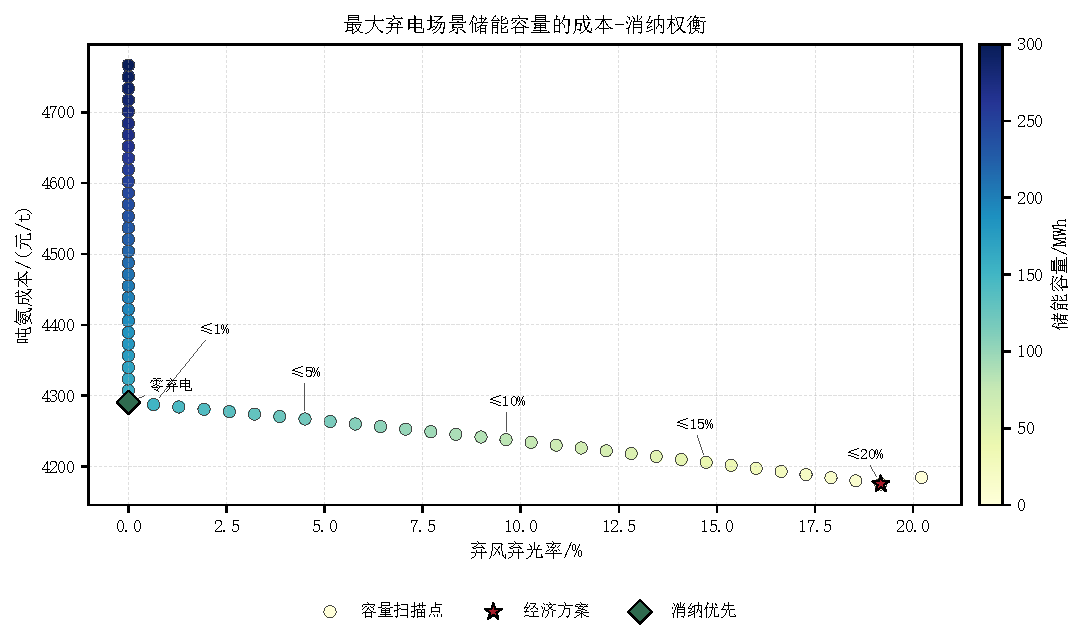
\includegraphics[width=0.86\textwidth]{fig05_q4_storage_pareto.pdf}
  \caption{最大弃电场景储能容量的成本--消纳权衡}
  \label{fig:q4_pareto}
\end{figure}

为量化公共电网的平衡支撑价值，本文以离网+储能方案的各场景日产氨量为目标，求并网同产量调度。单位产品支撑价值定义为
\[
v^{grid}=\frac{C^{off+bat,year}-C^{grid,year}}{M^{\NHthree,year}}.
\]
计算得
\[
v^{grid}=4046.47-3310.66=735.81\ \text{元/t}.
\]
该值可理解为公共电网为园区提供备用、互济和余电消纳服务所体现的单位产品经济价值。

\begin{figure}[H]
  \centering
  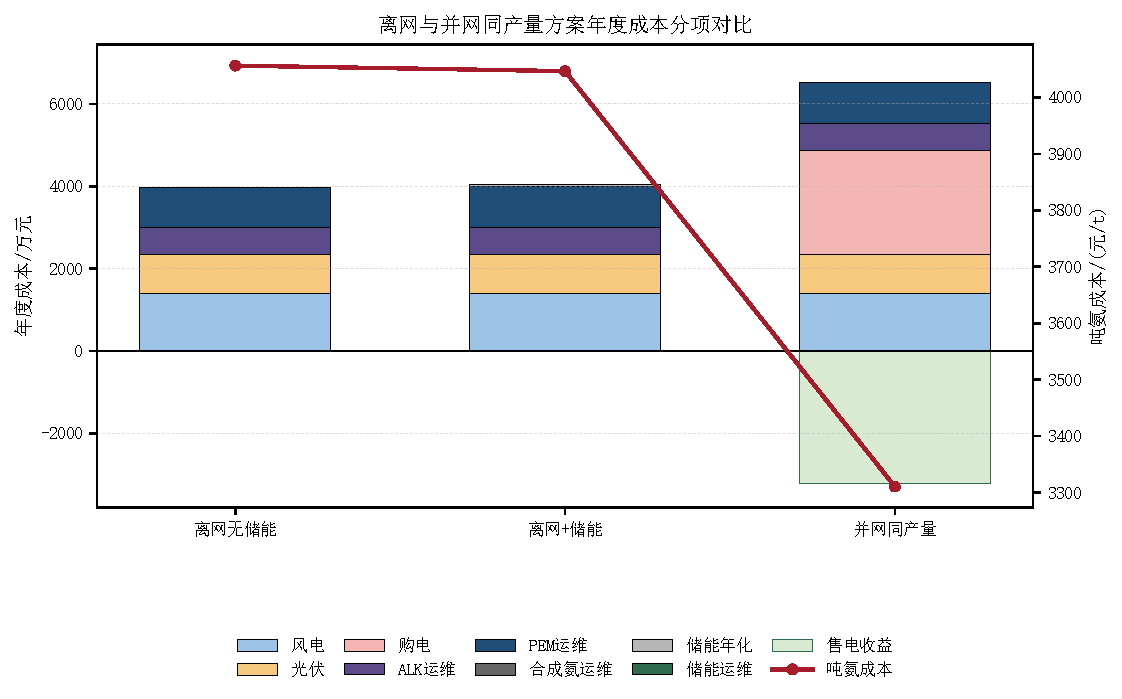
\includegraphics[width=0.78\textwidth]{fig06_q4_mode_cost_breakdown.pdf}
  \caption{离网与并网同产量的成本分项对比}
  \label{fig:q4_mode_cost}
\end{figure}

\section{问题五：绿电直连高渗透影响分析}

\subsection{证据矩阵构建}

问题五不再建立新的调度模型，而是从前四问提取数值证据，形成“模型依据--系统影响--政策含义”的分析链条。核心证据见表\ref{tab:q5_evidence}。

\begin{table}[H]
\centering
\caption{前四问支撑问题五的关键证据}
\label{tab:q5_evidence}
\scriptsize
\begin{tabular}{c p{0.12\textwidth} p{0.48\textwidth} p{0.25\textwidth}}
\toprule
编号 & 来源 & 数值证据 & 政策含义\\
\midrule
E1 & Q1 & 上网比例35.92\%，同时购电172.04 MWh、上网216.77 MWh & 应考核小时级源荷匹配\\
E2 & Q2 & 36 t/d成本最低但0天全满足，72 t/d全满足270天但成本最高 & 运行考核不能只看吨成本\\
E3 & Q3 & 36 t/d连续调节较离散开停降本284.35元/t，购电和上网均减少16216.93 MWh & 应重视柔性负荷价值\\
E4 & Q3 & 72 t/d上网比例7.05\%，36 t/d上网比例35.76\% & 新能源装机应以荷定源\\
E5 & Q4 & 离网无储能产能利用率37.74\%，5 MWh储能后缺供为0 & 离网需评估可靠性与储能\\
E6 & Q4 & 公共电网支撑价值735.81元/t & 并网项目应承担系统费用\\
E7 & Q4 & 满产逐小时自治需1156.31 MW至3006.39 MW装机 & 完全离网满产成本高\\
E8 & Q4 & 5 MWh为经济方案，80 MWh满足弃电率不超过10\%，155 MWh零弃电 & 储能需多目标评估\\
\bottomrule
\end{tabular}
\end{table}

\subsection{系统影响与政策建议}

绿电直连园区的有利影响主要体现在三方面：第一，高耗能绿氢绿氨负荷能够吸收本地风光电量，促进新能源就近消纳；第二，连续可调电解槽和合成氨装置可作为需求侧资源，降低公共电网购售电波动；第三，储能与柔性负荷组合有助于提升离网或弱联网场景下的可靠性。

同时，绿电直连高渗透也会带来风险。若项目只追求最低吨氨成本，可能选择低产量运行，导致上网比例升高并增加外部电网消纳压力。并网型项目若不承担系统运行费、备用和辅助服务费用，可能将平衡成本转移给公共电网。完全离网虽然强化物理绿电属性，但需要更大储能和冗余装机，经济性与土地资源约束突出。

\begin{figure}[H]
  \centering
  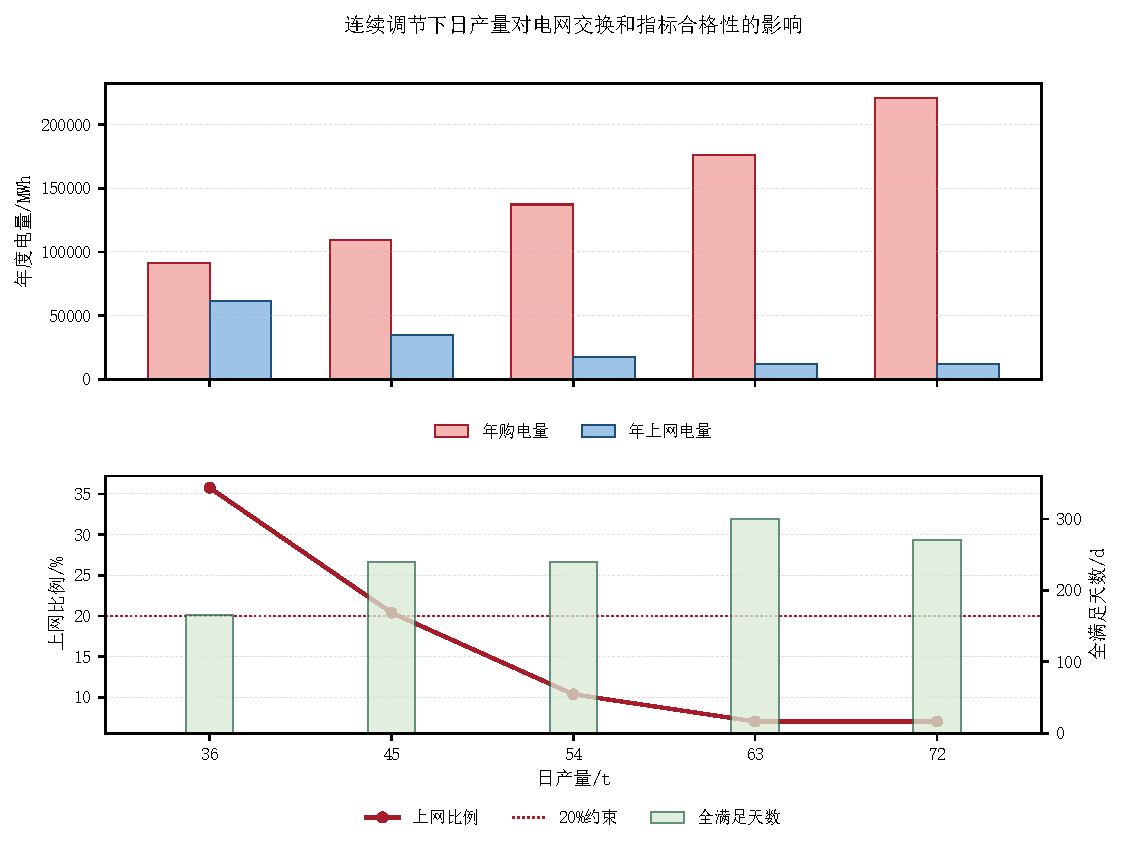
\includegraphics[width=0.82\textwidth]{fig07_q5_policy_evidence.pdf}
  \caption{连续调节下日产量对电网交换和指标合格性的影响}
  \label{fig:q5_policy_evidence}
\end{figure}

据此提出六条建议：建立小时级绿电溯源与分表计量制度；将上网比例、最大交换功率和反送时段纳入运行考核；把柔性负荷能力作为准入、评价和补偿对象；建立储能配置的经济性、弃电率和可靠性多目标评估；完善并网型项目的输配电费、系统运行费、备用和辅助服务费用分担机制；推进风光氢氨醇一体化与弱联网示范。

\section{结果汇总与综合讨论}

前四问的结果表明，绿电直连型电氢氨园区的运行优化并非单纯追求最低吨氨成本。问题一显示，刚性满负荷生产下虽然绿电比例较高，但上网比例超标。问题二说明，降低日产量可降低成本，却会削弱新能源就地消纳。问题三表明，连续负荷率调节在相同产量下可进一步降低成本并提高指标合格天数，是改善源荷匹配的关键柔性手段。问题四则表明，离网运行需要储能和冗余容量支撑，公共电网的平衡服务具有可量化经济价值。

从工程决策角度看，若以典型场景合规为目标，54 t/d是问题二和问题三中较均衡的日产量方案；若以全年全满足天数最大为目标，问题三中63 t/d表现最好；若以离网可靠性为目标，5 MWh储能可消除常规负荷缺供，但若追求低弃电或零弃电，则需显著提高储能容量。由此可见，绿电直连项目应在吨氨成本、产能利用率、绿电指标、弃电率和电网支撑成本之间进行综合权衡。

\section{模型评价与推广}

本文模型的主要优点是：第一，将绿电直连三项政策指标贯穿五问，避免只做电量成本优化；第二，构建了从刚性基准到离散调节、连续调节、离网储能和政策影响的统一递进链条；第三，问题三和问题四均引入互斥二进制变量，避免购售电套利和储能同时充放电；第四，给出了公共电网支撑价值和储能经济--消纳Pareto权衡，使模型结果具有政策解释能力。

模型局限也较明确。真实Haber-Bosch合成氨系统受温度、压力、循环气和催化剂寿命约束，不能像一般电负荷一样快速波动；本文未显式配置氢储罐和氨储罐，因而低估了电氢氨系统内部物料缓冲能力；吨氨成本未纳入题面未给出的电解槽、空分、压缩和储氢储氨投资；风光不确定性仅按24个代表场景处理，未考虑连续极端天气和预测误差。

后续可在当前模型基础上加入负荷爬坡率、启停成本和最小开停时间：
\[
0.1z_t\le u_t\le z_t,\quad
v_t\ge z_t-z_{t-1},\quad
-R^{down}\le u_t-u_{t-1}\le R^{up}.
\]
也可引入氢储罐动态
\[
H_t=(1-\rho^H)H_{t-1}+Q^{H2,prod}_t-Q^{H2,use}_t,
\]
或采用CVaR刻画场景风险：
\[
\min \sum_sp_sC_s+\lambda\left[\eta+\frac{1}{1-\alpha}\sum_sp_s\xi_s\right],
\quad \xi_s\ge C_s-\eta.
\]
进一步结合配电网潮流、电压约束、辅助服务市场和绿证碳价机制，可将本文模型推广为源网荷储氢氨协同规划与运行评估工具。

\section{结论}

本文围绕绿电直连型电氢氨园区建立了统一的小时级优化分析框架。主要结论如下：

\begin{enumerate}[label=(\arabic*)]
  \item 刚性满负荷制氨下，典型日新能源自发自用比例为64.08\%，总用电量绿电比例为69.21\%，但上网比例为35.92\%，不满足不超过20\%的要求，说明固定负荷存在显著源荷错配。
  \item 离散开停机能够降低运行成本，但低日产量方案会提高上网电量。典型场景中，若要求三项指标全部满足，54 t/d为最低成本离散方案。
  \item 连续负荷率调节相对离散开停机具有明显优势。36 t/d方案降本284.35元/t，全满足天数由0天提高至165天；45 t/d全满足天数由15天提高至240天。
  \item 离网运行下当前风光装机难以支撑高利用率生产。5 MWh储能可消除常规负荷缺供并降低弃电，但若要求最大弃电场景弃电率不超过10\%，需80 MWh储能；若要求零弃电，需155 MWh储能。
  \item 并网同产量方案的年均吨氨成本为3310.66元/t，离网+储能为4046.47元/t，公共电网支撑价值为735.81元/t，说明并网型绿电直连项目应合理承担系统平衡费用。
  \item 政策上应坚持小时级源荷匹配、以荷定源、柔性负荷补偿、储能多目标评估和系统费用分担，促进新能源消纳、产业脱碳和电力系统安全协调统一。
\end{enumerate}

\begin{thebibliography}{99}
\bibitem{policy_green_direct_2026}
国家发展改革委，国家能源局. 关于有序推动多用户绿电直连发展有关事项的通知[Z]. 2026.

\bibitem{policy_green_direct_2025}
国家发展改革委，国家能源局. 关于有序推动绿电直连发展有关事项的通知[Z]. 2025.

\bibitem{policy_market_price}
国家发展改革委，国家能源局. 关于深化新能源上网电价市场化改革 促进新能源高质量发展的通知[Z]. 2025.

\bibitem{policy_renewable_substitution}
国家发展改革委等. 关于大力实施可再生能源替代行动的指导意见[Z]. 2024.

\bibitem{policy_source_grid_load_storage}
国家发展改革委，国家能源局. 关于推进电力源网荷储一体化和多能互补发展的指导意见[Z]. 2021.

\bibitem{irena_ammonia}
International Renewable Energy Agency. Innovation Outlook: Renewable Ammonia[R]. 2022.

\bibitem{iea_hydrogen}
International Energy Agency. Global Hydrogen Review[R]. 2025.

\bibitem{eu_rfnbo}
European Commission. Commission Delegated Regulation (EU) 2023/1184[R]. 2023.
\end{thebibliography}

\appendix

\section{附录A：代码与结果文件说明}

主要求解脚本包括问题一至问题五的\texttt{solve\_q1.py}、\texttt{solve\_q2.py}、\texttt{solve\_q3.py}、\texttt{solve\_q4.py}和\texttt{solve\_q5.py}。公共模块\texttt{model\_common}负责参数管理、数据读取、指标计算和统一绘图风格。所有数值结果来自各问\texttt{outputs}目录中的CSV文件和Markdown摘要，图件同时保存为PNG、PDF和SVG格式。

\begin{table}[H]
\centering
\caption{主要输出文件索引}
\small
\begin{tabular}{p{0.16\textwidth}p{0.72\textwidth}}
\toprule
问题 & 主要输出 \\
\midrule
Q1 & \begin{tabular}[t]{@{}l@{}}\texttt{q1\_summary.csv}，\texttt{q1\_hourly\_results.csv}，图1--图5\end{tabular} \\
Q2 & \begin{tabular}[t]{@{}l@{}}\texttt{q2\_typical\_summary.csv}，\texttt{q2\_annual\_summary.csv}，图1--图7\end{tabular} \\
Q3 & \begin{tabular}[t]{@{}l@{}}\texttt{q3\_annual\_summary.csv}\\ \texttt{q3\_compare\_q2\_summary.csv}，图1--图8\end{tabular} \\
Q4 & \begin{tabular}[t]{@{}l@{}}\texttt{q4\_storage\_pareto\_summary.csv}\\ \texttt{q4\_mode\_comparison\_summary.csv}，图1--图6\end{tabular} \\
Q5 & \begin{tabular}[t]{@{}l@{}}\texttt{q5\_model\_evidence\_summary.csv}\\ \texttt{q5\_policy\_recommendation\_matrix.csv}\end{tabular} \\
\bottomrule
\end{tabular}
\end{table}

\section{附录B：数值校验说明}

问题三连续调节模型校验显示，最大功率平衡误差为$1.42\times10^{-14}$ MW，同时购电与售电小时数为0，日产量约束误差为$1.42\times10^{-14}$ t。问题四离网模型校验显示，无储能与有储能功率平衡最大误差均为$7.11\times10^{-15}$ MW，储能SOC动态最大误差为$6.66\times10^{-15}$ MWh，储能同时充放电乘积最大值为$6.35\times10^{-14}$，均为数值优化容差量级。

\section{附录C：未放入正文的补充材料}

由于正文页数限制，本文未在正文中展示所有场景热力图、成本箱线图、年度成本分布曲线和小时级调度明细。这些图表和数据均保存在各问\texttt{outputs}文件夹中，可用于复核具体场景运行机理。支撑材料压缩包建议包含代码、CSV结果、Markdown摘要和论文所用图件，不包含自动生成的\texttt{\_\_pycache\_\_}目录和临时文件。

\end{document}
